\chapter{Introduction} \label{ch:introduction}

The JEGA library contains two global optimization methods. The first
is a Multi-objective Genetic Algorithm (MOGA) which performs Pareto
optimization.  This is the primary deliverable of the JEGA software.
The second is a Single-objective Genetic Algorithm (SOGA) which
performs optimization on a single objective function or a weighted
sum of multiple objectives. Both methods support general
constraints, a mixture of real and discrete variables, and a variety
of objective types. The JEGA library was written by John Eddy,
currently a principal member of the technical staff in the System
Readiness and Sustainment Technologies department at Sandia National
Laboratories, Albuquerque, New Mexico.

\section{Motivation for JEGA Development} \label{sec:JEGA_motivation}
The following quote from the DAKOTA 5.3 User's
Manual~\cite{DUM:13:2013} briefly describes the motivation for
optimization in general.

\vspace{1em}
\begin{center}
\parbox{5in}{ \emph{``Computational models are commonly used in
engineering design and scientific discovery activities for simulating
complex physical systems in disciplines such as fluid mechanics,
structural dynamics, heat transfer, nonlinear structural mechanics,
shock physics, and many others. These simulators can be an enormous
aid to engineers who want to develop an understanding and/or predictive
capability for complex behaviors typically observed in the corresponding
physical systems. Simulators often serve as virtual prototypes, where
a set of predefined system parameters, such as size or location
dimensions and material properties, are adjusted to improve the
performance of a system, as defined by one or more system performance
objectives. Such optimization or tuning of the virtual prototype
requires executing the simulator, evaluating performance objective(s),
and adjusting the system parameters in an iterative, automated, and
directed way. System performance objectives can be formulated, for
example, to minimize weight, cost, or defects; to limit a critical
temperature, stress, or vibration response; or to maximize performance,
reliability, throughput, agility, or design robustness.''} }
\end{center}
\vspace{1em}

Of particular interest to the JEGA project are those problems that
have multiple objectives.  See Section~\ref{sec:general_MOP} for a
detailed discussion of multi-objective optimization problems (MOPs).
Such problems are very commonly encountered in optimization. Quoting
from~\cite{coello:eas_for_mop:2002}:

\begin{center}
\parbox{5in}{ \emph{``Problems with multiple objectives arise in a
natural fashion in most disciplines and their solution has been a
challenge to researchers for a long time.''} }
\end{center}

The solutions to multi-objective problems can provide a decision
maker with a great deal of information about how the various
objectives relate to one another including the trade-offs that must
occur when choosing a final solution.  This will be discussed
further in Section~\ref{sec:general_MOP} when the form of the
solutions to these problems is discussed.

\textcolor[rgb]{1.00,0.00,0.00}{ One of the primary motivations for
the development of JEGA has been to provide engineers with a
systematic means of obtaining improved or optimal designs using
their simulator-based models. Making this capability available to
engineers generally leads to better designs and improved system
performance at earlier stages of the design phase, and eliminates
some of the dependence on real prototypes and testing, thereby
shortening the design cycle and reducing overall product development
costs.}

The next section discusses both single and multiple objective
optimization problems in mathematical detail.

\section{Optimization Problems} \label{sec:general_MOP}
The standard form single objective optimization problem (SOP) is
shown in Equation~\ref{eq:general_SOP}.

\begin{eqnarray} \label{eq:general_SOP}
\nonumber minimize: & & \\
\nonumber F(\bar{x}) \\
\nonumber & & \\
\nonumber subject\; to: & & \\
          g_i(\bar{x}) &\leq & 0\quad i=1,2,...,m \\
\nonumber h_i(\bar{x}) &=& 0\quad i=1,2,...,p \\
\nonumber x_{li} \leq & x_i & \leq x_{ui}
\end{eqnarray}

Where $\bar{x}$ is a vector of design variables, $F$ is a scalar
function or composition of functions resulting in a scalar value,
$g$ are inequality constraints, $h$ are equality constraints, and
the variables may be bounded.  The fact that $F$ is scalar indicates
that this is a single objective problem.

As stated, the primary deliverable of JEGA is a multi-objective
genetic optimizer which operates on multi-objective optimization
problems.  The general form of an MOP is shown in
Equation~\ref{eq:general_MOP} below.

\begin{eqnarray} \label{eq:general_MOP}
\nonumber minimize: & & \\
\nonumber \bar{F}(\bar{x}) &=& [f_1(\bar{x}), f_2(\bar{x}), ..., f_k(\bar{x})]^T \\
\nonumber & & \\
\nonumber subject\; to: & & \\
          g_i(\bar{x}) &\leq & 0\quad i=1,2,...,m \\
\nonumber h_i(\bar{x}) &=& 0\quad i=1,2,...,p \\
\nonumber x_{li} \leq & x_i & \leq x_{ui}
\end{eqnarray}

The difference between Equation~\ref{eq:general_SOP} and
Equation~\ref{eq:general_MOP} is that in
Equation~\ref{eq:general_MOP}, the objective function is vector
valued.

When the objective function in a problem is vector valued, there is
the potential for a vector valued solution.  The existence of such a
solution depends on the relationships that exists between the
objectives. The three possible relationships between any two
objectives are as follows:

\begin{enumerate}
    \item Cooperative - This is the relationship that exists if the
    two objectives share design variables and are not in competition
    with one another.  This means that the two objectives desire the
    same trends in the shared design variables and that improvement
    of one objective typically accompanies improvement of the other.

    \item Competitive - This is the relationship that exists if the
    two objectives share design variables and are not cooperative
    with one another.  This means that the two objectives desire a
    different trend for at least one of the shared variables and
    that improvement of one typically accompanies worsening of the
    other.

    \item Indifferent - This is the relationship that exists if the
    two objectives have no design variables in common.  In this
    case, the two objectives move independently of one another.  The
    problem may be effectively solved by carrying out two separate
    single objective optimizations depending on the form of any shared
    constraints or may be solved using an appropriate
    weighted-sum-of-objectives scheme.
\end{enumerate}

The case of indifferent objectives is quite un-interesting from a
multi-objective optimization viewpoint because it does not require
true multi-objective optimization and it can generally be detected
prior to any analysis or optimization.  This case can be expressed
using set notation as follows:
\begin{equation}\label{eq:indifference}
    f_1(\bar{x}_1\subseteq{\bar{x}}),f_2(\bar{x}_2\subseteq{\bar{x}}):\bar{x}_1 \cap
    \bar{x}_2=\varnothing
\end{equation}

\noindent where $\bar{x}$ is the set of all design variables used
throughout the entire problem, $\bar{x}_1$ is the subset of
$\bar{x}$ used by objective 1, and $\bar{x}_2$ is the subset of
$\bar{x}$ used by objective 2. In this equation, $\bar{x}$ has
components $\bar{x}=\{x_1,x_2,x_3...x_n\}$ where n is the total
number of design variables.

The case in which all objectives are cooperative is more interesting
than that of indifference because it is often not possible to detect
this situation prior to the optimization.  However, the result of
solving a problem such as this will generally be a single superior
solution or a set of solutions with the exact same superior
performance characteristics.

The case in which two or more of the objectives in a multi-objective
problem are in competition with one another is by far the most
interesting from a multi-objective optimization viewpoint.  It is in
this case that the solution will no longer be a single superior
design point but instead will be a set, possibly infinite in size,
of efficient solutions called the \emph{Pareto optimal
set}~\cite{pareto:manuale:1906}.

The Pareto optimal set is the collection of all Pareto optimal
solutions. A Pareto optimal solution is one that is efficient or
non-dominated in the set of all possible solutions where the
criteria for dominance is given in Equation~\ref{eq:dominance}
below.

A feasible performance vector $\bar{u}=\{u_1,u_2,u_3...u_k\}$
dominates a feasible performance vector
$\bar{v}=\{v_1,v_2,v_3...v_k\}$ (denoted $\bar{u} \preceq \bar{v}$)
iff $\bar{u}$ is partially less than $\bar{v}$.
\begin{equation}\label{eq:dominance}
    \forall i \in
    \{1,...,k\},u_i \leq v_i\wedge \exists i \in \{1,...,k\},u_i < v_i
\end{equation}
\noindent where k is the total number of objectives each of which is
to be minimized.

Equation~\ref{eq:dominance} states that in order for one design to
dominate another it must be better with respect to at least one
objective and no worse with respect to all others.

The Pareto optimal set is then given by Equation~\ref{eq:pareto_set}
below.
\begin{equation}\label{eq:pareto_set}
    P^*:=\{\bar{x}\in\Omega\mid\neg\exists\bar{x}'\in\Omega\quad
         \bar{F}(\bar{x}')\preceq\bar{F}(\bar{x})\}
\end{equation}
\noindent where $\Omega$ is the set of all feasible solutions to the
problem~\cite{coello:eas_for_mop:2002}.

Equation~\ref{eq:pareto_set} states that the Pareto optimal set is
defined as the set of all feasible solutions for which there are no
other feasible solutions that dominate them, or more simply, every
solution that is non-dominated in the entire feasible space.

Plotting the Pareto optimal set in the performance space displays
the Pareto frontier which is a portion of the boundary of the
feasible space such that all points on the region are Pareto optimal
as shown in Figure~\ref{fig:pareto_front} below.  The blue line in
the figure is the Pareto frontier.

\begin{figure}[!ht]
    \centering
    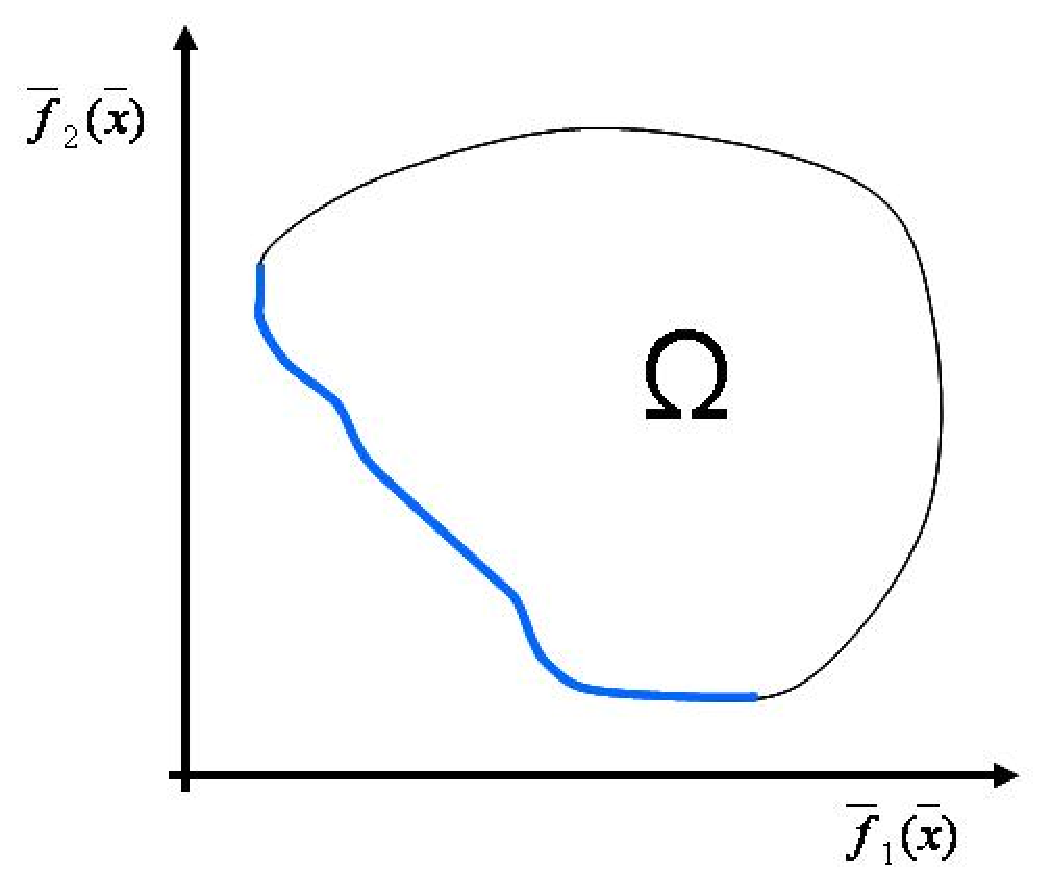
\includegraphics[scale=0.45]{../../images/pareto_front.eps}
    \caption{The Typical Looking Pareto Frontier.}
    \label{fig:pareto_front}
\end{figure}

As can be seen from the figure, having a representation of the
Pareto frontier can not only provide a decision maker with a variety
of possible efficient solutions, but it can also provide a designer
with information about the trade-offs that exist between objectives.
For example, with such a curve, a designer can answer questions
like:

\vspace{1em}
\begin{center}
\parbox{5in}{ \emph{"From my current candidate solution, how much of objective 1
would I have to sacrifice to achieve a corresponding improvement of
X\% in objective 2?"}}
\end{center}
\vspace{1em}

There is a vast body of research involving techniques for solving
single objective optimization problems.  The options for solving
multiple objective problems are considerably more limited.  Problems
such as these can be difficult to solve.  Often, multi-objective
optimization problems are converted into single objective problems
for the purpose of solution.  There are a number of ways to do this
including various weighted sum schemes, the normal boundary
intersection (NBI) method~\cite{das:nbi:1998}, goal programming,
utility theoretical methods, etc.  Generally, such techniques
require the repeated solution of the resulting single objective
problem using different problem parameters in order to generate a
sampling of the Pareto optimal set.  Each of these techniques
suffers from certain drawbacks generally caused by a sensitivity to
the shape of the Pareto frontier~\cite{dennis:weight_sum_drawbacks:1997}.

JEGA employs a genetic algorithm to solve these sorts of problems.
the advantages of using evolutionary algorithms for solving such
problems are many.  They include:


\begin{itemize}

\item insensitivity to the shape of the Pareto frontier;
\item intrinsic maintenance of a set of solutions;
\item solution to the problem in a single optimization;
\item potential for global solutions; and
\item zeroth order operations.

\end{itemize}

There are also disadvantages to using evolutionary algorithms for
solving optimization problems such as:

\begin{itemize}

\item a need for a large number of objective function and constraint function evaluations;
\item no guarantee of optimality nor any indication of degree of optimality of a solution;
\item no guarantee of achieving the same solution on subsequent runs of the algorithm.

\end{itemize}



\section{Capabilities of JEGA} \label{sec:JEGA_capabilities}

JEGA is highly configurable and is therefore very flexible both at
run time and at compile time. In addition, it is easily extensible
such that new algorithmic components can be inserted with few or no
changes to the core code.

\section{How Does JEGA Work} \label{sec:JEGA_how_it_works}

JEGA can easily be used as a library by other programs or as a stand
alone application.  The advantage to the stand alone approach is
that only your evaluation code would have to be written and compiled
instead of re-compiling and/or relinking JEGA.  The disadvantage is
that communication between JEGA and the evaluation code takes place
through the file system which is many orders of magnitude slower
than the direct interface possible when using JEGA as a library.

\section{Using This Manual} \label{sec:JEGA_using_manual}
